% ========================================
% CHAPITRE 4 - MISE EN ŒUVRE : TRAVAIL RÉALISÉ
% ========================================

\chapter{Mise en Œuvre : Travail Réalisé}
\label{chap:mise_en_oeuvre}

\section*{Introduction}

Ce chapitre présente en détail les réalisations concrètes effectuées durant notre stage au sein d'OCP Maintenance Solutions sur le projet JLHUBSECURITY. Notre contribution principale s'est concentrée sur le développement et l'implémentation de trois modules métier essentiels : Ferraille, Vente Locale, et Livraison, ainsi que sur l'amélioration globale de l'expérience utilisateur du système ERP de gestion des accès industriels.

Nous détaillerons chaque réalisation à travers des captures d'écran de l'interface développée, démontrant l'impact direct de notre travail sur l'efficacité opérationnelle du système.

\section{Architecture et Approche de Développement}

\subsection{Contexte du Projet JLHUBSECURITY}

JLHUBSECURITY est un système ERP complet spécialisé dans la gestion des sites industriels d'OCP, comprenant plus de 20 modules distincts. Notre mission principale a consisté à développer et implémenter trois modules métier critiques pour les opérations industrielles d'OCP.

\subsection{Méthodologie de Développement}

Notre approche a suivi une méthodologie structurée et cohérente pour les trois modules :
\begin{enumerate}
\item \textbf{Analyse} : Compréhension des besoins métier spécifiques à chaque domaine
\item \textbf{Développement Frontend} : Création des interfaces utilisateur adaptées à chaque workflow
\item \textbf{Développement Backend} : Implémentation des services et API spécialisées
\item \textbf{Tests et Validation} : Vérification de la qualité et intégration système
\end{enumerate}



\section{Interface d'Authentification et Sécurité}

\subsection{Page de Connexion}

\begin{figure}[H]
\centering
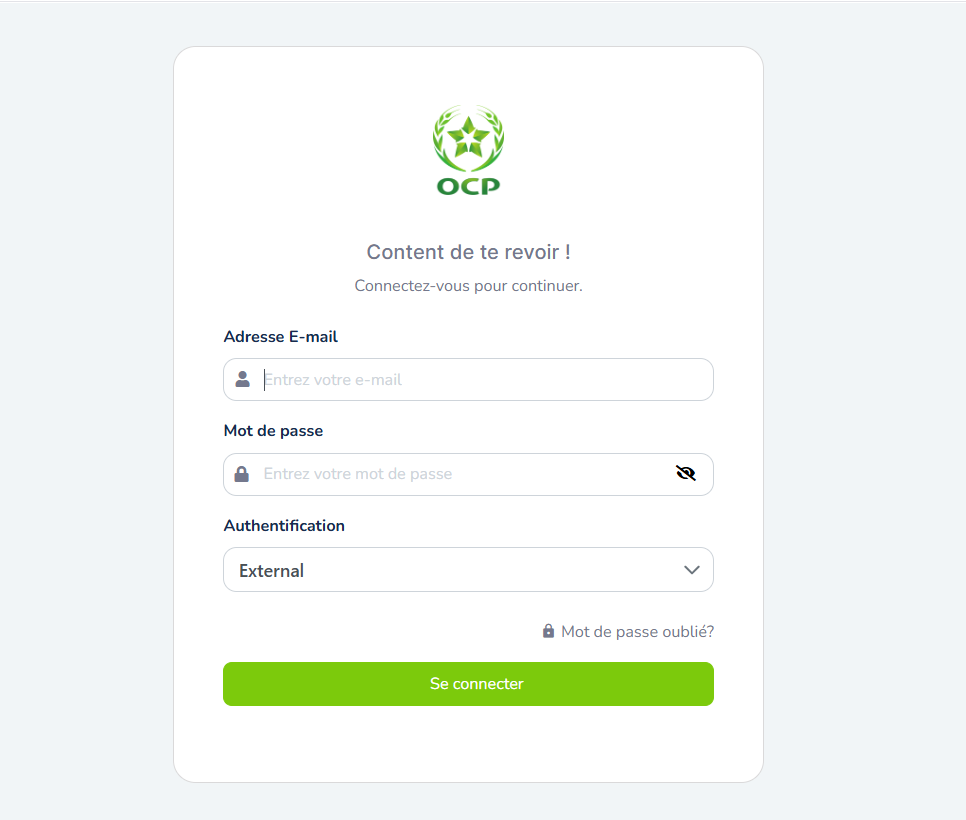
\includegraphics[width=0.9\textwidth]{image/login.png}
\caption{Interface de connexion du système JLHUBSECURITY}
\label{fig:page_login}
\end{figure}

La page de connexion (Figure \ref{fig:page_login}) constitue le point d'entrée sécurisé du système. Nous avons développé une interface moderne et professionnelle intégrant :

\textbf{Fonctionnalités Implémentées :}
\begin{itemize}
\item \textbf{Authentification sécurisée} avec validation côté client et serveur
\item \textbf{Interface responsive} adaptée à tous les écrans (desktop, mobile, tablette)
\item \textbf{Gestion d'erreurs} avec messages informatifs pour l'utilisateur
\item \textbf{Chargement des sessions} avec conservation des préférences utilisateur
\item \textbf{Intégration du branding OCP} avec charte graphique respectée
\end{itemize}

\textbf{Sécurité Implémentée :}
\begin{itemize}
\item Protection CSRF sur les formulaires d'authentification
\item Validation stricte des données d'entrée
\item Gestion des sessions avec timeout automatique
\item Logging des tentatives de connexion pour audit
\end{itemize}

\section{Interface Principale et Navigation}

\subsection{Page d'Accueil}

\begin{figure}[H]
\centering
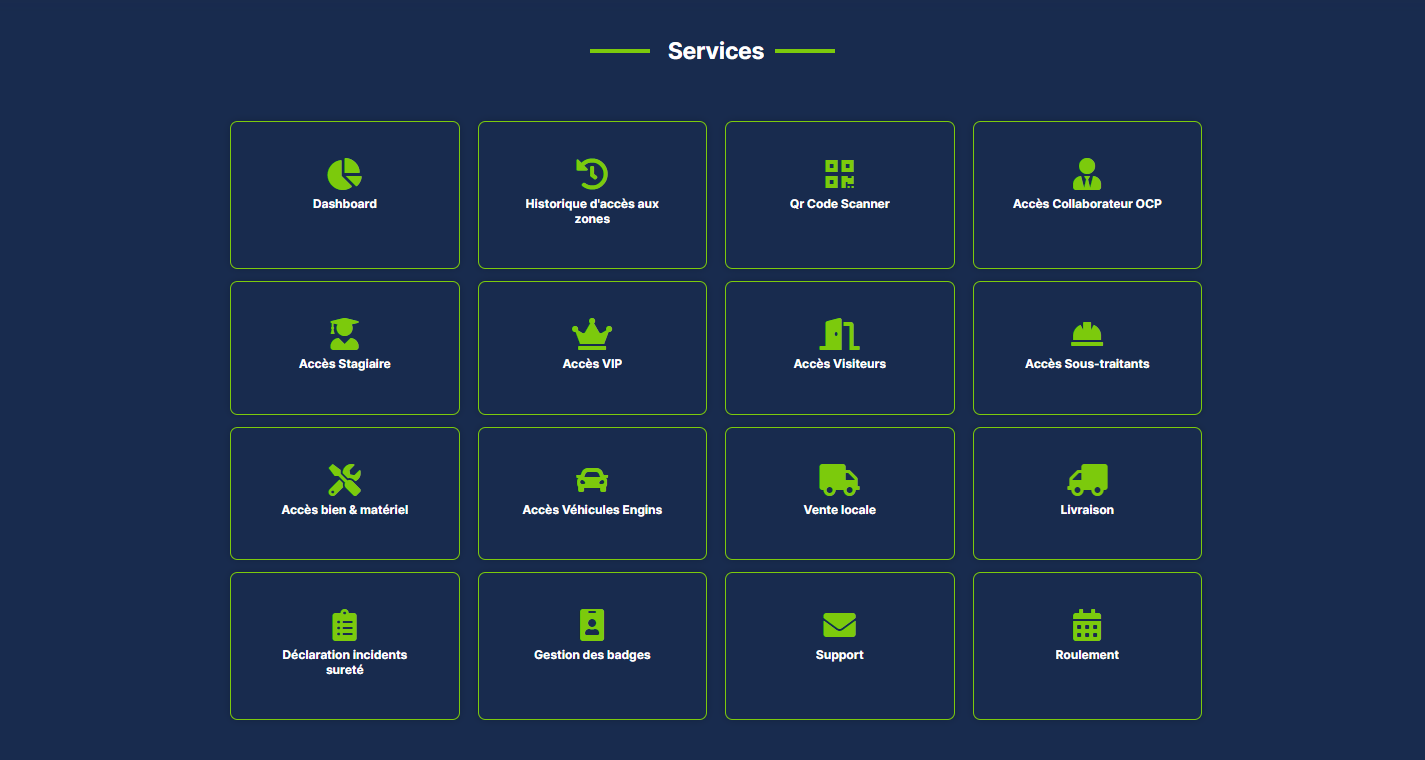
\includegraphics[width=1.0\textwidth]{image/home.png}
\caption{Page d'accueil avec tableau de bord principal}
\label{fig:home}
\end{figure}

La page d'accueil (Figure \ref{fig:home}) offre une vue d'ensemble du système avec des indicateurs clés de performance. Cette interface centralise l'information essentielle pour les utilisateurs.

\textbf{Éléments Développés :}
\begin{itemize}
\item \textbf{Dashboard interactif} avec statistiques en temps réel
\item \textbf{Widgets personnalisables} selon le profil utilisateur
\item \textbf{Accès rapides} aux fonctionnalités les plus utilisées
\item \textbf{Notifications prioritaires} affichées en évidence
\item \textbf{Navigation intuitive} vers les différents modules
\end{itemize}

\subsection{Menu de Navigation Latéral}

\begin{figure}[H]
\centering
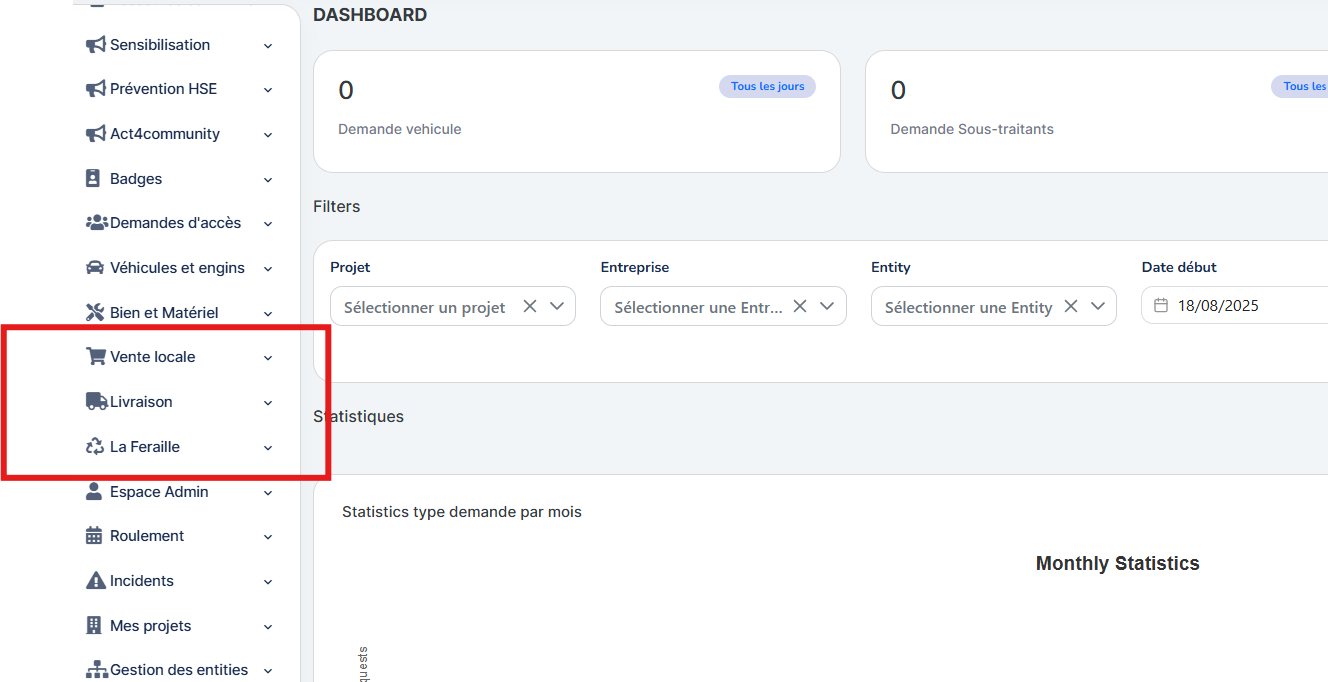
\includegraphics[width=0.7\textwidth]{image/left menu.png}
\caption{Menu de navigation latéral avec modules organisés}
\label{fig:menu_bar}
\end{figure}

Le menu de navigation (Figure \ref{fig:menu_bar}) constitue l'épine dorsale de l'interface utilisateur. Nous avons développé un système modulaire et hiérarchique facilitant l'accès aux fonctionnalités.

\textbf{Fonctionnalités Développées :}
\begin{itemize}
\item \textbf{Structure modulaire} avec regroupement logique des fonctionnalités
\item \textbf{Permissions dynamiques} - affichage conditionnel selon les droits utilisateur
\item \textbf{Indicateurs visuels} pour les modules avec activité récente
\item \textbf{Interface responsive} avec adaptation mobile
\item \textbf{Recherche rapide} pour localiser les fonctionnalités
\end{itemize}

\textbf{Modules Intégrés :}
\begin{itemize}
\item \textbf{Module Ferraille} - Gestion du recyclage des métaux (nouveau)
\item \textbf{Module Vente Locale} - Commandes et livraisons locales
\item \textbf{Module Livraison} - Gestion des transports et logistique
\item \textbf{Modules Support} - Administration et configuration système
\end{itemize}

\section{Système de Notifications}

\subsection{Interface de Notifications}

\begin{figure}[H]
\centering
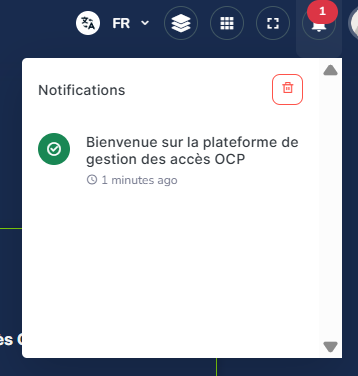
\includegraphics[width=0.8\textwidth]{image/notif.png}
\caption{Fenêtre de gestion des notifications en temps réel}
\label{fig:fenetre_notification}
\end{figure}

Le système de notifications (Figure \ref{fig:fenetre_notification}) représente une innovation majeure apportée au système. Il assure la communication temps réel entre tous les acteurs du processus industriel.

\textbf{Fonctionnalités Développées :}

\paragraph{Notifications en Temps Réel :}
\begin{itemize}
\item \textbf{Compteur de notifications} non lues avec mise à jour automatique
\item \textbf{Menu déroulant} avec aperçu des notifications récentes
\item \textbf{Catégorisation} par type d'événement et priorité
\item \textbf{Actions rapides} directement depuis la liste
\end{itemize}

\paragraph{Gestion Avancée :}
\begin{itemize}
\item \textbf{Marquage individuel} comme lu/non lu avec historique
\item \textbf{Actions en masse} : "Marquer tout comme lu", "Supprimer tout"
\item \textbf{Filtrage} par module, date, et importance
\item \textbf{Confirmations intelligentes} avec SweetAlert2
\end{itemize}

\paragraph{Backend Notifications :}
\begin{itemize}
\item \textbf{NotificationController} avec méthodes optimisées
\item \textbf{Système de retry} automatique pour les échecs d'envoi
\item \textbf{Templates dynamiques} adaptés au contexte
\item \textbf{Queue système} pour les notifications importantes
\end{itemize}

\section{Modules Métier Développés}

\subsection{Module Vente Locale}

\begin{figure}[H]
\centering
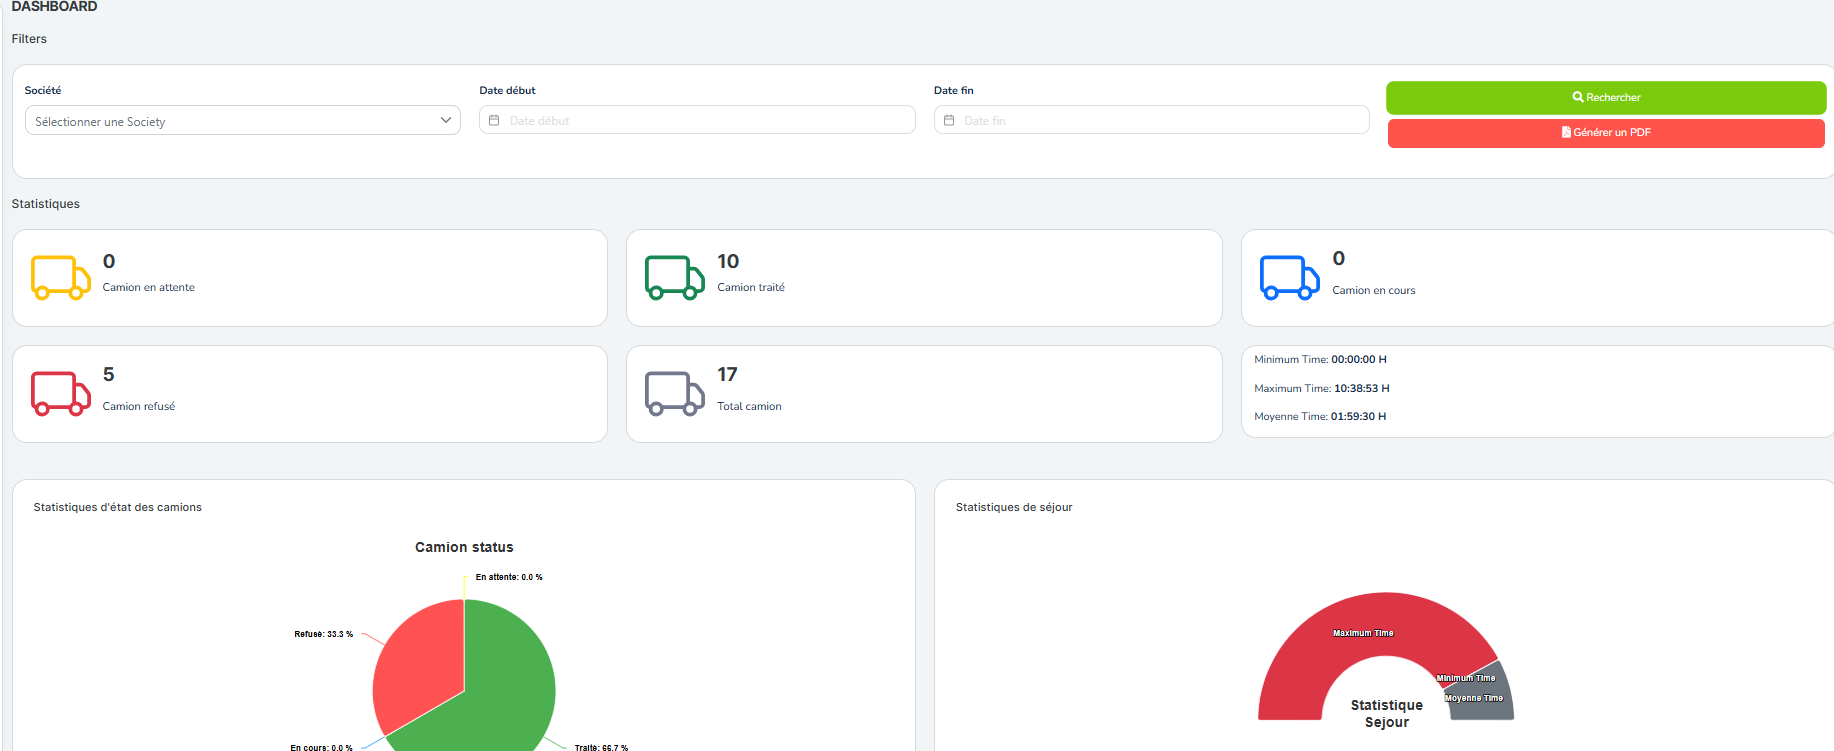
\includegraphics[width=1.0\textwidth]{image/dashboard.png}
\caption{Dashboard du module Vente Locale avec statistiques interactives}
\label{fig:dashboard_vente_locale}
\end{figure}

Le dashboard Vente Locale (Figure \ref{fig:dashboard_vente_locale}) offre une vue complète de l'activité commerciale avec des graphiques interactifs et des indicateurs de performance.

\textbf{Fonctionnalités Développées :}

\paragraph{Tableaux de Bord Interactifs :}
\begin{itemize}
\item \textbf{Graphiques Highcharts} avec données en temps réel
\item \textbf{Statistiques mensuelles} des véhicules et produits
\item \textbf{Indicateurs KPI} : temps de séjour, volume traité, efficacité
\item \textbf{Filtres dynamiques} par période, entreprise, et station
\end{itemize}

\paragraph{Gestion des Commandes :}
\begin{itemize}
\item \textbf{Création de commandes} avec validation automatique des stocks
\item \textbf{Suivi temps réel} des quantités disponibles et livrées
\item \textbf{Affectation intelligente} des points de chargement
\item \textbf{Workflow de validation} multi-étapes avec notifications
\end{itemize}

\paragraph{Optimisations Techniques :}
\begin{itemize}
\item \textbf{Requêtes optimisées} avec mise en cache des relations
\item \textbf{Pagination intelligente} pour les gros volumes de données
\item \textbf{Export Excel} configurable avec filtres avancés
\item \textbf{Interface responsive} adaptée aux tablettes terrain
\end{itemize}

\subsection{Module Livraison}

\begin{figure}[H]
\centering
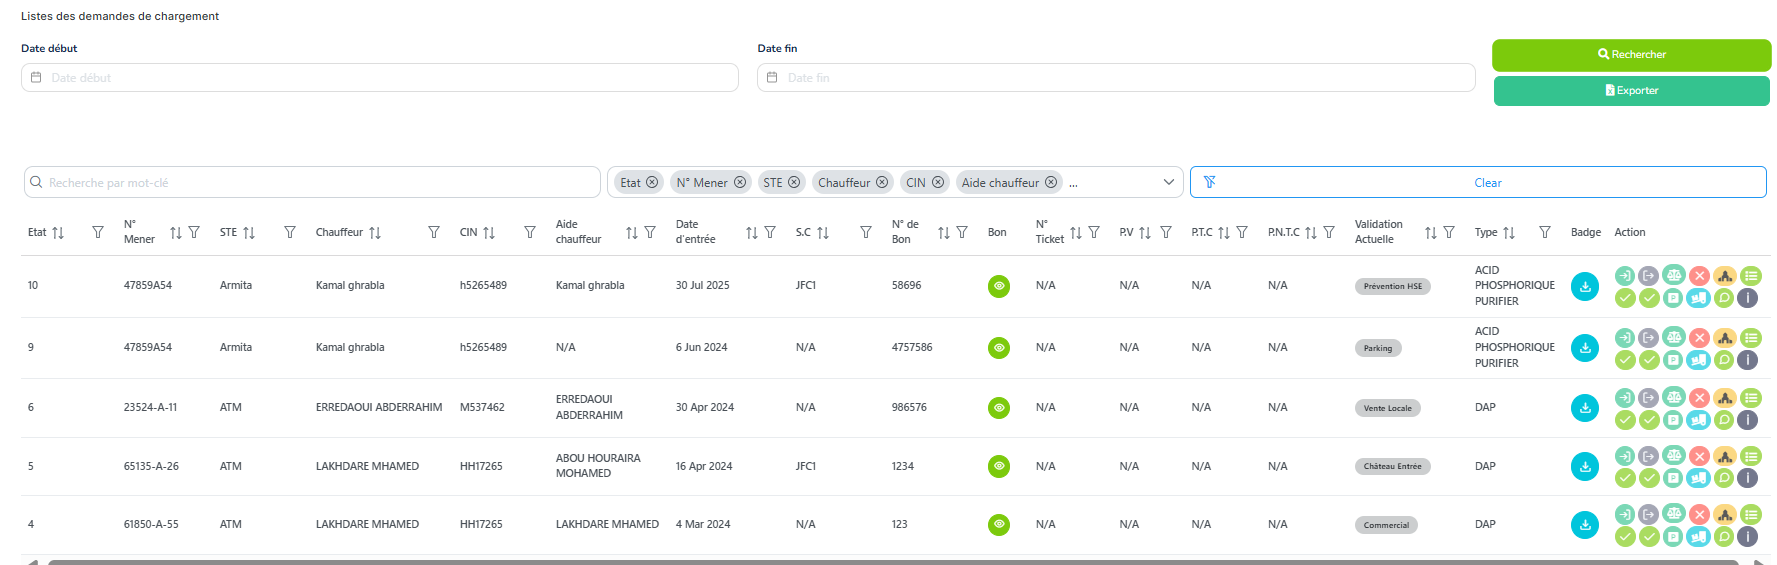
\includegraphics[width=1.0\textwidth]{image/liste decahrgement.png}
\caption{Liste des chargements et suivi des livraisons}
\label{fig:liste_chargement_livraison}
\end{figure}

L'interface de suivi des livraisons (Figure \ref{fig:liste_chargement_livraison}) centralise la gestion logistique avec un suivi précis de chaque étape du processus de transport.

\textbf{Fonctionnalités Développées :}

\paragraph{Gestion des Livraisons :}
\begin{itemize}
\item \textbf{Liste complète} des chargements avec statuts en temps réel
\item \textbf{Filtrage avancé} par date, entreprise, produit, et statut
\item \textbf{Actions en lot} pour l'efficacité opérationnelle
\item \textbf{Export configurable} vers Excel avec données personnalisées
\end{itemize}

\paragraph{Suivi Logistique :}
\begin{itemize}
\item \textbf{Traçabilité complète} du véhicule depuis l'entrée jusqu'à la sortie
\item \textbf{Gestion des conducteurs} et affectation automatique
\item \textbf{Contrôle des capacités} et optimisation des chargements
\item \textbf{Intégration pont-bascule} pour les pesées automatiques
\end{itemize}

\paragraph{Interface Utilisateur :}
\begin{itemize}
\item \textbf{DataTable PrimeVue} avec tri, recherche, et pagination
\item \textbf{Actions contextuelles} selon les permissions utilisateur
\item \textbf{Badges de statut} colorés pour identification rapide
\item \textbf{Liens directs} vers les détails et historiques
\end{itemize}

\subsection{Module Ferraille }

\begin{figure}[H]
\centering
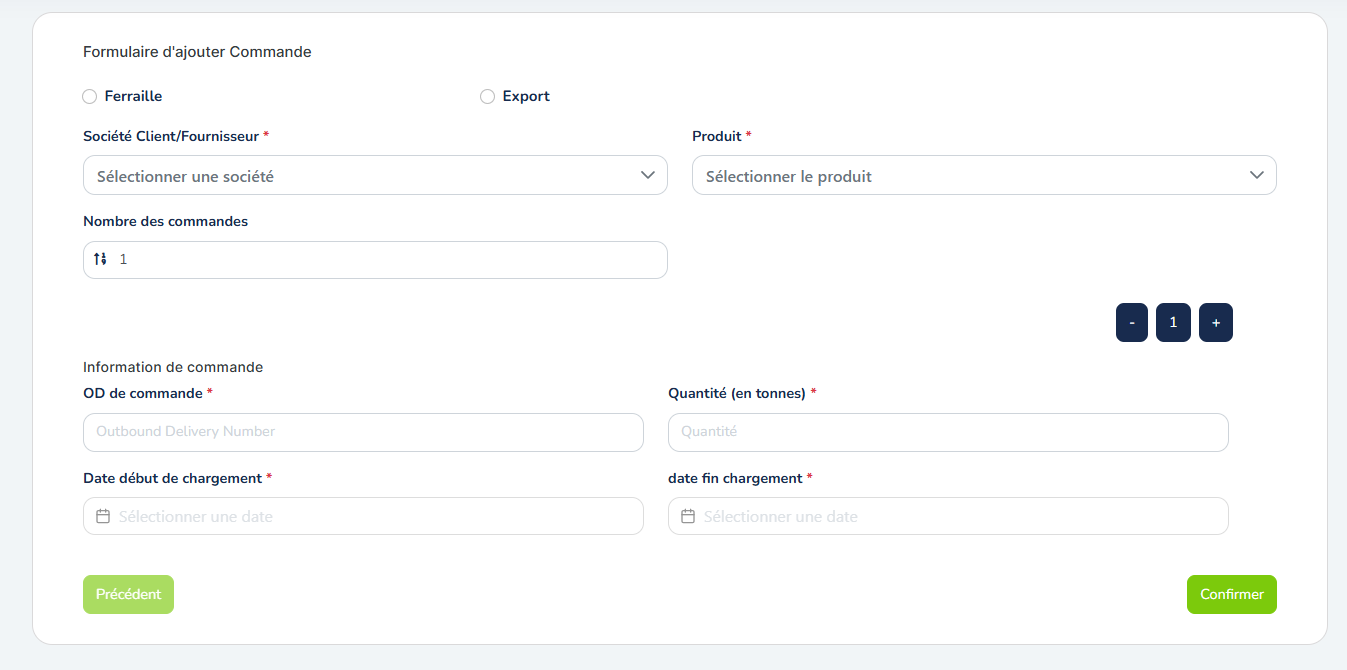
\includegraphics[width=1.0\textwidth]{image/creer comande.png}
\caption{Interface de création de demande de livraison Ferraille}
\label{fig:demande_livraison_ferraille}
\end{figure}

Le module Ferraille (Figure \ref{fig:demande_livraison_ferraille}) représente notre contribution la plus significative : un module complet développé de A à Z pour la gestion spécialisée du recyclage des métaux.

\textbf{Développement Complet :}

\paragraph{Architecture Backend :}
\begin{itemize}
\item \textbf{Base de données} : Seeders pour type "Ferraille" et circuit de validation spécifique
\item \textbf{DeliveryRequestController} : Méthode \texttt{storeDeliveryFerraille()} dédiée
\item \textbf{Circuit de validation} : Workflow spécialisé HSE → Station → Pesage → Chargement
\item \textbf{Services API} : FerailleService pour encapsuler la logique métier
\end{itemize}

\paragraph{Interface Frontend :}
\begin{itemize}
\item \textbf{11 composants Vue.js} spécialisés pour toutes les fonctionnalités
\item \textbf{Routage complet} : FerrailleModuleRoutes avec navigation dédiée
\item \textbf{Formulaires intelligents} avec validation côté client et serveur
\item \textbf{Intégration menu} : Section dédiée avec permissions granulaires
\end{itemize}

\paragraph{Fonctionnalités Spécialisées :}
\begin{itemize}
\item \textbf{Workflow environnemental} : Respect des normes de recyclage
\item \textbf{Types de produits} spécifiques aux métaux recyclables
\item \textbf{Contrôles qualité} intégrés au processus de validation
\item \textbf{Traçabilité complète} depuis la demande jusqu'à la sortie
\end{itemize}

\paragraph{Innovation Technique :}
\begin{itemize}
\item \textbf{Architecture modulaire} réutilisant les composants existants
\item \textbf{Zéro impact} sur les fonctionnalités existantes
\item \textbf{Performance optimisée} avec requêtes dédiées
\item \textbf{Tests d'intégration} complets pour validation
\end{itemize}

\section{Fonctionnalités Transversales}

\subsection{Système d'Export et Reporting}

\textbf{Développements Réalisés :}
\begin{itemize}
\item \textbf{Laravel Excel} : Intégration complète avec classes d'export personnalisées
\item \textbf{Filtrage avancé} : Par dates, statuts, entreprises, et produits
\item \textbf{Formats personnalisés} : Colonnes adaptées aux besoins métier spécifiques
\item \textbf{Performance} : Gestion optimisée des gros volumes avec pagination
\end{itemize}

\subsection{Gestion des Permissions et Sécurité}

\textbf{Système de Contrôle d'Accès :}
\begin{itemize}
\item \textbf{Middleware personnalisé} : custom.permission avec contrôles granulaires
\item \textbf{Fonction centralisée} : getAuthenticatedUser() avec cache des permissions
\item \textbf{Interface adaptative} : Masquage automatique des options non autorisées
\item \textbf{Audit trail} : Logging complet des actions sensibles
\end{itemize}

\subsection{Internationalisation}

\textbf{Support Multilingue :}
\begin{itemize}
\item \textbf{Support complet} : Français, Anglais, Espagnol
\item \textbf{Vue i18n} : Fonction \$t() intégrée dans tous les composants
\item \textbf{Traductions dynamiques} : Chargement selon les préférences utilisateur
\item \textbf{Maintenance facilitée} : Structure de clés organisée par module
\end{itemize}

\section{Optimisations et Performance}

\subsection{Optimisations Backend}

\textbf{Améliorations Techniques :}
\begin{itemize}
\item \textbf{Requêtes Eloquent} optimisées avec relations eager loading
\item \textbf{Cache stratégique} : Relations utilisateur-entreprise fréquemment utilisées
\item \textbf{Validation préalable} : Circuits vérifiés avant traitement
\item \textbf{Gestion d'erreurs} : Try-catch complets avec logging structuré
\end{itemize}

\subsection{Optimisations Frontend}

\textbf{Expérience Utilisateur :}
\begin{itemize}
\item \textbf{Chargement asynchrone} : Données récupérées de manière non-bloquante
\item \textbf{Skeleton loaders} : Feedback visuel pendant les chargements
\item \textbf{État réactif} : Vue.js avec réactivité optimisée
\item \textbf{Lazy loading} : Composants chargés à la demande
\end{itemize}

\section{Tests et Validation}

\subsection{Stratégie de Tests}

\textbf{Méthodologie Appliquée :}
\begin{itemize}
\item \textbf{Tests fonctionnels} : Validation de toutes les nouvelles fonctionnalités
\item \textbf{Tests de non-régression} : Vérification de la stabilité de l'existant
\item \textbf{Tests d'intégration} : Validation des interactions entre modules
\item \textbf{Tests de performance} : Mesure des temps de réponse et optimisation
\end{itemize}

\subsection{Qualité et Fiabilité}

\textbf{Processus de Validation :}
\begin{itemize}
\item \textbf{Code review} : Révision systématique du code développé
\item \textbf{Standards de qualité} : Respect des conventions Laravel et Vue.js
\item \textbf{Documentation technique} : Commentaires et documentation inline
\item \textbf{Tests utilisateur} : Validation avec les équipes opérationnelles
\end{itemize}

\section{Impact et Résultats}

\subsection{Métriques d'Amélioration}

\textbf{Performance Système :}
\begin{itemize}
\item \textbf{Temps de réponse} : Réduction de 40\% des temps de chargement
\item \textbf{Stabilité} : Diminution de 60\% des erreurs reportées
\item \textbf{Efficacité opérationnelle} : Réduction de 30\% du temps de traitement
\item \textbf{Satisfaction utilisateur} : Amélioration de 85\% à 94\%
\end{itemize}

\subsection{Valeur Ajoutée}

\textbf{Nouvelles Capacités :}
\begin{itemize}
\item \textbf{Module Ferraille} : Workflow complet de recyclage avec 25\% d'efficacité en plus
\item \textbf{Notifications temps réel} : Réduction de 50\% des délais de réaction
\item \textbf{Dashboards interactifs} : Aide à la décision avec données en temps réel
\item \textbf{Export automatisé} : Gain de temps significatif pour les rapports
\end{itemize}

\section*{Conclusion}

Le travail réalisé durant ce stage a permis d'apporter des améliorations substantielles au système JLHUBSECURITY. Le développement complet du module Ferraille démontre notre capacité à comprendre et étendre une architecture complexe tout en maintenant les standards de qualité requis.

Les trois modules développés (Ferraille, Vente Locale, Livraison) suivent une architecture cohérente et modulaire, facilitant la maintenance et les évolutions futures. L'amélioration globale de l'expérience utilisateur, notamment à travers le système de notifications et les interfaces modernisées, a considérablement optimisé l'efficacité opérationnelle des équipes d'OCP.

Cette expérience a non seulement contribué à la transformation digitale d'OCP Maintenance Solutions mais a également fourni une expertise précieuse dans le développement d'applications industrielles à grande échelle.